\documentclass[xcolor=svgnames,dvipsnames,table, hyperref=pdftex, mathserif, presentation]{beamer}
\usepackage{amsmath,amssymb,amsfonts,amsthm}
\usepackage{ctex}
\setCJKsansfont{KaiTi}% 文泉驿的黑体
\usepackage{graphics}
\usepackage{graphicx}
\usepackage{xcolor}
\usepackage{wasysym}
\usepackage{bbm}
\usepackage{url}
\usepackage{beamerleanprogress}
\usepackage{tikz-dependency}
\usepackage{tikz-qtree}

\usetheme{CambridgeUS}
%\usetheme{Pittsburgh}
\usecolortheme{orchid} % seahorse  orchid rose
\setbeamertemplate{blocks}[rounded][shadow=true]
\AtBeginSection[]{%
  \begin{frame}<beamer>
    \frametitle{Outline}
      \tableofcontents[current] 
    \end{frame}
  \addtocounter{framenumber}{-1}% If you don't want them to affect the slide number
}
\AtBeginSubsection[]
{
  \begin{frame}
  \frametitle{Outline}
    \tableofcontents[currentsection,currentsubsection]
  %\tableofcontents[sectionstyle=show/hide,subsectionstyle=hide/show/hide]
  \end{frame}
  \addtocounter{framenumber}{-1}% If you don't want them to affect the slide number
}
\newcommand{\setof}[1]{\ensuremath{\left \{ #1 \right \}}}
\newcommand{\tuple}[1]{\ensuremath{\left \langle #1 \right \rangle }}
\newcommand{\red}[1]{\textcolor{red}{#1}}
\newcommand{\brown}[1]{\textcolor{brown}{#1}}
\newcommand{\green}[1]{\textcolor{green}{#1}}
\newcommand{\blue}[1]{\textcolor{blue}{#1}}
\newcommand{\cyan}[1]{\textcolor{cyan}{#1}}

%gets rid of navigation symbols
%\setbeamertemplate{navigation symbols}{}

\begin{document}

\title[MF+FOL]{Injecting Logical Background for Relation Extraction}

\institute[icst.wip@pku]{
  
}
\author[Tim Rockt]{
  Tim Rockt aschel (UCL)\\
  Sameer Singh (UW)\\
  Sebastian Riedel (UCL)\\ 
}

\frame[t,plain]{ \titlepage } % [t,plain]

\frame{
  \frametitle{ Outline  }
  
   \begin{itemize}
      \item 论文概述
      \item 矩阵分解(Matrix factorization), 一阶谓词逻辑(first-order logic)
      \item 符号集(Notation)
      \item 一阶谓词逻辑注入(Inject)矩阵分解
	  \begin{itemize}
	   \item 矩阵分解之前操作(Pre-Factorization)
	   \item 融入矩阵分解之中('joint')
	  \end{itemize}

      \item 实验
	  \begin{itemize}
	   \item 预处理,规则生成,评价
	  \end{itemize}
   \end{itemize}

}

\frame{
  \frametitle{ summary }
  \centering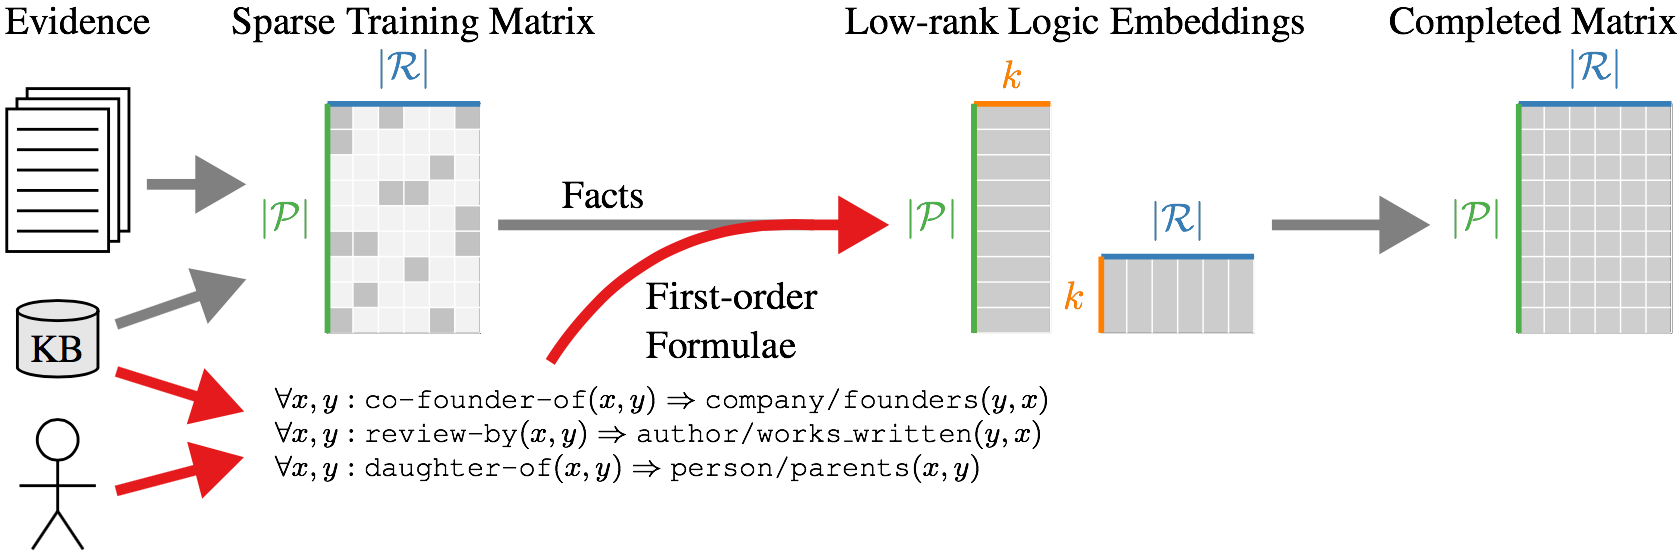
\includegraphics[width=0.9\hsize]{file/overview.png}
}
\end{document}